 \graphicspath{ {Figs/Chapter4/} }
 
 \chapter{Implementación de un Modelo de red Blockchain}
 
 Con la finalidad de ilustrar la aplicabilidad de la tecnología {\it blockchain} a procesos administrativos universitarios, 
 %cumplir los objetivos trazados, 
 se implementó un modelo de red básico, siguiendo los pasos propuestos en el capítulo anterior. El modelo provee las estructuras necesarias para desarrollar un flujo de trabajo asociado a la transcripción de materias utilizados en universidades. Particularmente, este modelo de red está inspirado en el caso de uso denominado \textit{Creación de Transcripciones} del sistema SIGPAE (Sistema de Gestión de Programas Analíticos de Estudio) de la Universidad Simón Bolívar, que se encuentra actualmente en fase de desarrollo. No obstante, este modelo de red propone funciones y actores adicionales al caso original de SIGPAE, con el propósito de demostrar más ampliamente las características útiles e integrables a este tipo de procesos admiistrativos.
 %presentar una mayor cantidad de características útiles e integrables en el flujo de trabajo del caso de uso anteriormente identificado.
 
 
Para la  implementación del modelo de red se utilizó la herramienta \textit{Hyperledger Composer} versión 0.19.10, usando el lenguaje de programación Javascript versión \textit{ECMAScript5} (para la implementación de la lógica transaccional), el lenguaje de modelado  \textit{Composer CTO} (para definir el modelo de recursos) y el lenguaje  \textit{Compose ACL} (para definir la permisología). Finalmente, para la interacción y prueba de la red se hizo uso de la herramienta \textit{Hyperledger Composer Playground}. 
 
En el capítulo anterior, se describe minuciosamente el proceso de creación del modelo de red \textit{blockchain}. A continuación, se procede a presentar la aplicación de dicho procesos en el diseño e implementación de un modelo de red específico.

\section{Planteamiento del problema y requerimientos}

El proyecto SIGPAE tiene como uno de sus objetivos permitir la transcripción y actualización  de los contenidos programáticos de cada curso o materia que conforman los programas de estudio de la Universidad Simón Bolívar. El proceso consiste en la transcripción digital de un programa de estudio existente(avalado por la coordinacion,departamento o dependencia responsable),la cual es realizada por un transcriptor designado, posteriormente es verificada por un supervisor de transcripción y finalmente es aprobada por DACE(Direccion de Admision y Control de Estudios) una vez comprobada la completitud de la transcripcion. En este contexto, se pretende  crear una plataforma que provea las estructuras necesarias para gestionar lo concerniente al flujo de trabajo relacionado a transcripciones de los contenidos programáticos. 

%El problema identificado, se resume en la necesidad de la creación de una plataforma que provea las estructuras necesarias para gestionar lo concerniente al flujo de trabajo relacionado a transcripciones de programas de estudio. 

Por ende, el modelo de red debe estar diseñado para soportar los siguientes requerimientos:

\begin{itemize}
    \item Permitir la iniciación o creación de una transcripción por parte de los participantes.
    \item Permitir la edición de una transcripción  y actualización de su estado por parte de los participantes.
    \item Manejo de revisiones y observaciones sobre la transcripciones por parte de los participantes.
    \item Gestión de validación y aprobación de la transcripciones por parte de los participantes.
    \item Gestión de accesos y permisos que restrinja las acciones y recursos que pueden ser accedidos por los participantes dentro del flujo de trabajo.
\end{itemize}

Los recursos propuestos para el modelo de red se dividen en:

\textbf{Participantes}
\begin{itemize}
    \item Proponente: da inicio a una transcripción y le asigna un supervisor.
    \item Transcriptor: encargado de realizar la edición de la transcripción.
    \item Supervisor: revisa y valida las transcripciones para su aprobación final.
    \item Auditor: encargado de aprobar transcripciones o enviar observaciones con modificaciones sugeridas para su aprobación.
\end{itemize}

\textbf{Activos} 
\begin{itemize}
    \item Transcripción: elemento o activo del sistema que representa una transcripción de un programa de estudio que aún no se encuentra avalado.
    \item Programa: elemento o activo del sistema que funciona como instancia de un programa de estudio avalado por la USB.
\end{itemize}

\textbf{Transacciones} 
\begin{itemize}
    \item TranscriptorAsignado: asigna un Transcriptor a una \textit{Transcripción}.
    \item SupervisorAsignado: determina la asignación de un supervisor a una Transcripción.
    \item RevisionTranscripcion: ejecuta el envío (guardado) de una revisión con modificaciones sugeridas a una \textit{Transcripcion}. 
    \item ObservacionTranscripcion: ejecuta la operación de enviar (guardar) observaciones a una \textit{Transcripción} necesarias para su aprobación final.
    \item ValidarTranscripcion: efectúa la validación de una \textit{Transcripción}.
    \item AprobarTranscripcion: efectúa la aprobación de una \textit{Transcripción}
\end{itemize}

\section{Diseño y Modelado}
 Se diseñó un diagrama BPMN (por sus siglas en inglés {\it Business Process Model Notation}), que permite identificar el flujo de trabajo sobre una transcripción, las transacciones que se realizan y los participantes involucrados. 
 
 \begin{figure}[H]
    \centering
    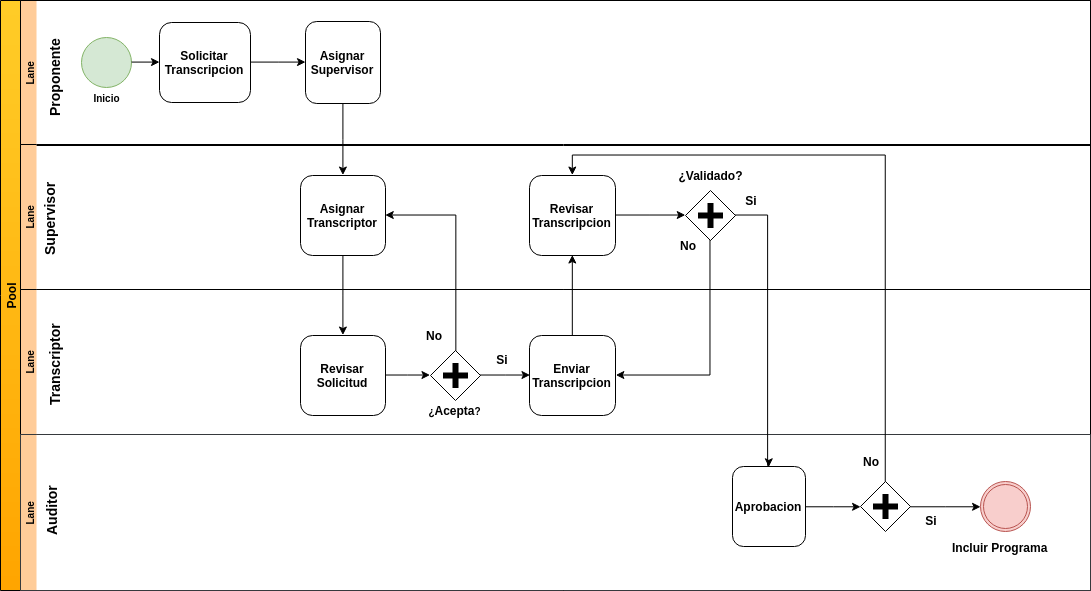
\includegraphics[width=1\textwidth]{flujo_transcripcion.png}
    \caption{Flujo de trabajo de una transcripción}
    \label{flujo_trabajo}
\end{figure}
 

A continuación, se procede a describir los pasos del flujo de trabajo necesarios para la creación de un activo Transcripción, según lo mostrado en la Figura~\ref{flujo_trabajo}.
\begin{enumerate}
    \item El Proponente da inicio al proceso solicitando la creación de una Transcripción.
    \item El Proponente asigna un Supervisor a la Transcripción, una vez iniciado el proceso.
    \item El Supervisor designa un Transcriptor y le envía una solicitud de participación.
     \item Si el Transcriptor acepta la solicitud, se inicia la fase de edición y éste puede empezar a transcribir el programa. De lo contrario, se retorna al paso 3.
     \item El Transcriptor envía la Transcripción para su revisión una vez terminada la edición.
     \item El Supervisor revisa la Transcripción y la valida en caso de estar completa y correcta para iniciar la fase de aprobación. De ser necesaria una modificación, el Supervisor enviará las sugerencias necesarias para su validación y se vuelve al paso 5.
     \item El Auditor realiza una revisión final de la Transcripción. Si ésta cumple todos los requisitos, es aprobada e incluida como programa oficial. De lo contrario, el Auditor procede a enviar observaciones con modificaciones necesarias y se retorna al paso 6.
\end{enumerate}

\section {Implementación y desarrollo}

Finalmente, se presentan los 3 componentes principales que conforman el modelo de red expuestos en el capítulo anterior, que se definen en 3 tipos de archivos. En este capítulo se presenta la estructura del código desarrollado. El código completo se encuentra en el Apéndice A. 
%Por simplicidad el código completo desarrollado se encuentran expuestos en el apartado final de este proyecto y se procede a explicar su estructura.

\subsection{Modelo de Recursos}

%\textcolor{blue}{CORRECION SUGERIDA: Explicación de cuadros de todo el capitulo  }
Este modelo se encuentra descrito en el archivo \textit{programas-academicos.cto} que está incluido en el Apéndice A.
%la sección de \textit{Anexos de Código}. 

A continuación se detallan todos los recursos definidos en este archivo con sus respectiva descripción de atributos y tipos.

\textbf{Participantes}

En el Cuadro \ref{tabla:proponente} se especifica los atributos del  \textit{Proponente}. Se utiliza únicamente el nombre ya que el proponente puede ser una persona particular, una coordinación o dependencia de la universidad interesada en la transcripción de un programa.

\begin{table}[H]
    \captionsetup{justification=raggedleft}
    \caption{\textit{participant Proponente}}
    \centering
    \begin{tabular}{ |c|c|c| }
        \hline
        \textbf{Campo} & \textbf{Tipo} & \textbf{Descripcion} \\ 
             \hline
             participantId & String     & identificador del participante.\\
             nombre        & String     & nombre o alias del participante. \\
             rolAcademico & String & representa la figura académica del participante\\
        \hline
    \end{tabular}
    \label{tabla:proponente}
\end{table}


En el Cuadro \ref{tabla:transcriptor} se presentan los atributos del  Transcriptor el cual debe ser una persona particular, por ejemplo un estudiante, profesor, ayudante académico, entre otros.

\begin{table}[H]
    \caption{\textit{participant Transcriptor}}
    \centering
        \begin{tabular}{ |c|c|c| }
            \hline
            \textbf{Campo} & \textbf{Tipo} & \textbf{Descripción} \\
                 \hline
                 participantId & String     & identificador del participante.\\
                 nombre        & String     & nombre  del participante. \\
                 apellido      & String     & apellido del participante.\\
                 rolAcademico & String & representa la figura académica del participante.\\
                 \hline
        \end{tabular}
    \label{tabla:transcriptor}
\end{table}

En el Cuadro \ref{tabla:supervisor} se presentan los atributos del Supervisor, este debe ser una persona particular y debe tener cierto rango dentro de la comunidad universitaria por ejemplo un profesor.

\begin{table}[H]
    \caption{\textit{participant Supervisor}}
    \centering
     \begin{tabular}{ |c|c|c| }
        \hline
        \textbf{Campo} & \textbf{Tipo} & \textbf{Descripción} \\
             \hline
             participantId & String     & identificador del participante.\\
             nombre        & String     & nombre  del participante. \\
             apellido      & String     & apellido del participante.\\
             rolAcademico & String & representa la figura académica del participante.\\
             \hline
        \end{tabular}
    \label{tabla:supervisor}
\end{table}

En el Cuadro \ref{tabla:auditor} se presentan los atributos del Auditor, el cual debe ser asumido por  una dependencia de la universidad y no una persona particular. Por ejemplo una coordinación, departamento o decanato.

\begin{table}[H]
    \caption{\textit{participant Auditor}}
    \centering
    \begin{tabular}{ |c |c |c| }
        \hline
        \textbf{Campo} & \textbf{Tipo} & \textbf{Descripción} \\
             \hline
             participantId & String     & identificador del participante.\\
             denominacion        & String     & denominación o alias del participante. \\
             rolAcademico & String & representa la figura académica del participante.\\
             \hline
        \end{tabular}
    \label{tabla:auditor}
\end{table}



\textbf{Activos}

El Cuadro \ref{tabla:programa} muestra los atributos del activo Programa del modelo de red.  En la practica los contenidos programaticos (al cual hace referencia este activo) poseen mas atributos sin embargo por motivos de claridad del modelo estos se acotaron a los atributos principales.
\begin{table}[H]
    \caption{\textit{asset Programa}}
    \centering
     \begin{tabular}{ |c| c| c| }
        \hline
        \textbf{Campo} & \textbf{Tipo} & \textbf{Descripción} \\
             \hline    
             recursoId & String     & identificador del programa de estudio.\\
             denominacion & String & denominación o título del programa\\
             codigo & String & código asociado al programa de estudio\\
             contenido & String & contenido programático de la materia\\
             fechaElaboracion & DateTime & denominacion o Fecha de creacion del programa de estudio\\
             \hline
        \end{tabular}
    \label{tabla:programa}
\end{table}

%\textcolor{blue}{CORRECION PROPUESTA: Verificacion de la frase contenidos programaticos}

El activo \textit{Programa} fue incluido con motivos ilustrativos. El modelo de red se concentra en la gestión del activo \textit{Transcripción}.

El Cuadro \ref{tabla:transcripcion} muestra los atributos asociados al activo Transcripción del modelo de red.
Encontramos atributos especiales de tipo \textit{Transaction} o \textit{Transaction List} los cuales permiten asociar las transacciones u operaciones con el activo presentado.

\begin{table}[H]
    \caption{\textit{asset Transcripcion}}
    \centering
    \begin{tabular}{ |c |c |c| }
        \hline
        \textbf{Campo} & \textbf{Tipo} & \textbf{Descripción} \\
             \hline
             recursoId & String     & identificador del programa de estudio.\\
             denominacion & String & denominación o título del programa.\\
             codigo & String & código asociado al programa de estudio.\\
             contenido & String & contenido programático de la materia.\\
             estado & TranscripState & estado actual de una transcripción.\\
             transcriptorAsignado & Transaction &  referencia al transcriptor asociado.\\
             supervisorAsignado & Transaction & referencia al supervisor asociado.\\
             revisionesTranscrip & Transaction List & referencias a revisiones realizadas.\\
             observacionesTranscrip & Transaction List &  referencia a observaciones enviadas.\\
             fechaElaboracion & DateTime & fecha de creación de la propuesta de transcripción\\
             \hline
    \end{tabular}
    \label{tabla:transcripcion}
\end{table}

El campo \textit{estado} puede contener los valores \textit{ESPERA} , \textit{PENDIENTE}, \textit{APROBADO}.


A continuación se presenta en el Cuadro \ref{tabla:transacciones} las distintas transacciones definidas en el modelo con su descripción general.

\begin{table}[H]
    \centering
    \caption{\textit{Lista de Transactions}}
    \begin{tabular}{ |m{10em}|m{10em}|m{5em}| } 
        \hline
        \textbf{Transacción} & \textbf{Descripción} & \textbf {Campos} \\
            \hline
            TranscriptorAsignado &  operación de asignar un transcriptor & -\textit{Relation} transcriptor\\
            \hline
            SupervisorAsignado &  operacion de asignar un supervisor & -\textit{Relation} supervisor\\ 
            \hline
            RevisionTranscripcion &  operación que guarda una revisión en  transcripción & -\textit{String} revisión \\ 
            \hline
            ObservacionTranscripcion &  operación que guarda una observación en transcripción & -\textit{String} observación \\ 
            \hline
            ValidarTranscripcion &  operación que valida una edición  de transcripción y actualiza estado &  \\ 
            \hline
            AprobarTranscripcion & operación que aprueba una transcripción y actualiza estado &  \\ 
            \hline
    \end{tabular}
    \label{tabla:transacciones}
\end{table}

Todas las transacciones poseen una relación a Transcripción lo que permite  agregarlas dentro del registro del activo.

El campo \textit{Relation} en las transacciones \textit{TranscriptorAsignado} y \textit{SupervisorAsignado} permiten asociar al participante objetivo dentro del registro de la transacción.

El campo \textit{String} en las transacciones \textit{RevisionTranscripcion} y \textit{ObservacionTranscrip} permite guardar la revisión u observación dentro del registro de la transacción.

\subsection{Chaincodes o Lógica de transacciones}
La lógica de transacciones del modelo de red se encuentra definida   en funciones de Javascript, descritas en el archivo \textit{transcripcion.js} mostrado en detalle en el Apéndice A.
%incluido en la seccion de Anexos de Codigo. 

Se  presentan a continuación las funciones asociadas a las transacciones en el Cuadro \ref{tabla:chaincodes}.

 \begin{table}[H]
     \centering
          \caption{Chaincodes}
     \begin{tabular}{|m{10em}|m{22em}|}
         \hline
         Función & Descripción  \\
         \hline
         transcriptorAsignado & Actualiza el  campo \textit{transcriptorAsignado} de una transcripción con el transcriptor seleccionado \\
         \hline
         supervisorAsignado & Actualiza el campo \textit{transcriptorAsignado} de una transcripción con el supervisor seleccionado\\
         \hline
         revisionTranscripcion & Agrega una revisión en la lista asociada al  campo \textit{revisionesTranscripcion} de una transcripción \\
         \hline
         observacionTranscripcion & Agrega una observación a la lista asociada al campo \textit{observacionesTranscripcion} \\
         \hline
         validarTranscripcion & Actualiza el campo \textit{estado} de una transcripción con el valor \textit {PENDIENTE} indicando que la transcripción esta pendiente de aprobación\\
          \hline
         aprobarTranscripcion & Actualiza el campo \textit{estado} de una transcripción con el valor \textit{APROBADA} indicando que la transcripción fue aprobada y está pendiente su inclusión como programa de estudio.\\
         \hline
     \end{tabular}
     \label{tabla:chaincodes}
 \end{table}

No es necesario que las funciones tengan el mismo nombre que la transacciones encontradas en el archivo \textit{CTO}, sin embargo se recomienda utilizar esta práctica para mayor claridad.


\subsection{Lista de control de accesos}
Las reglas de  permisologia y accesos asociados a los recursos del modelo de red se describen en el archivo \textit{permission.acl} incluido en el Apéndice A.
%la seccion de Anexos de Codigo.

Se utilizó la siguiente nomenclatura para  nombrar las diferentes reglas del archivo \textbf{rule Participante\_Permisos\_Recurso}

Este patrón permite identificar y entender rápidamente el cometido de la regla. Por ejemplo, la regla:

\centerline{ \textit{rule Proponente\_RC\_Transcripcion}\{\} }   

Describe que el  participante  \textit{Proponente} tiene permisos  \textit{READ} y \textit{CREATE} (leer y crear), sobre el activo \textit{Transcripción}. 

En  los cuadros \ref{tabla:reglas_activos} y \ref{tabla:reglas_transacciones} se presentan los permisos sobre los activos y transacciones del modelo de red. En el primero se describen los accesos a los activos del modelo de red, y las acciones permitidas sobre este, quien puede ver, crear o realizar modificaciones sobre el activo mencionado. El segundo cuadro se exponen los participantes habilitados para la ejecución de las distintas transacciones del modelo.
 
\begin{table}[H]
    \centering
    \caption{Reglas definidas para los Activos del modelo de red}
    \begin{tabular}{|m{6em}|m{6em}|m{6em}|m{14em}|}
        \hline
            \multicolumn{4}{|c|}{Reglas sobre Activos}\\
        \hline
            \textbf{Activo} & \textbf{Participante(s)} & \textbf{Permiso(s)} & \textbf{Restricción}  \\
        \hline
            \multirow{2}{10em}{Transcripción} & Proponente & CREAR LEER & solo el proponente puede crear (iniciar) una transcripción \\
            & Transcriptor Supervisor Auditor & MODIFICAR LEER & todos menos el proponente puede modificar una transcripción.\\
        \hline
            Programa & Todos & LEER & todos los participantes pueden leer y visualizar un programa\\
        \hline
    \end{tabular}
    \label{tabla:reglas_activos}
\end{table}

\begin{table}[H]
    \centering
    \caption{Reglas definidas para las Transacciones del modelo de red}
    \begin{tabular}{|m{10em}|m{6em}|m{14em}|}
    \hline
        \multicolumn{3}{|c|}{Reglas sobre Transacciones}\\
    \hline
        \textbf{Transacción} & \textbf{Participante} & \textbf{Restricción}  \\
    \hline
         TranscriptorAsignado & Supervisor & sólo el supervisor puede asignar un transcriptor \\
         \hline
         SupervisorAsignado & Proponente & solo el proponente puede asignar un supervisor\\
         \hline
         RevisionTranscripcion & Auditor & solo el auditor puede hacer observaciones sobre una transcripción \\
         \hline
         ObservacionTranscripcion & Auditor & sólo el auditor puede hacer observaciones sobre una transcripción \\
         \hline
         ValidarTranscripcion & Supervisor& solo el supervisor puede validar un transcripción\\
         \hline
         AprobarTranscripcion & Auditor & solo el auditor puede aprobar una transcripción\\
    \hline
    \end{tabular}
    \label{tabla:reglas_transacciones}
\end{table}

\section{Interacción y prueba del modelo de red}

Para poder interactuar y probar el modelo de red, se utilizó la herramienta \textit{Composer Playground}. Como se definió en el capitulo anterior, esta herramienta provee una interfaz gráfica que permite probar el modelo de red, específicamente revisar los registros de recursos, probar transacciones e incluso implementar código que se ejecuta de manera inmediata. \textit{Composer Playground} puede ser utilizado con  una instalación local o a través de su aplicación en línea~\cite{composerPlayground}.

\textit{Hyperledger Composer} solo necesita los 3 archivos descritos en las secciones anteriores \textit{programas-academicos.cto}, \textit{transcripcion.js} y \text{permission.acl} para iniciar el modelo de red cómo se expone a continuación:

Se presenta la interfaz gráfica \textit{Playground}. La interfaz es bastante intuitiva y fácil de manejar, se concentra en la prueba de transacciones y verificaciones de registros definidos en el modelo de red. En la figura \ref{fig: playground-presentation} se aprecia una primera impresión de la interfaz donde es posible ver el histórico de transacciones realizadas hasta el momento.

\begin{figure}[H]
\centering
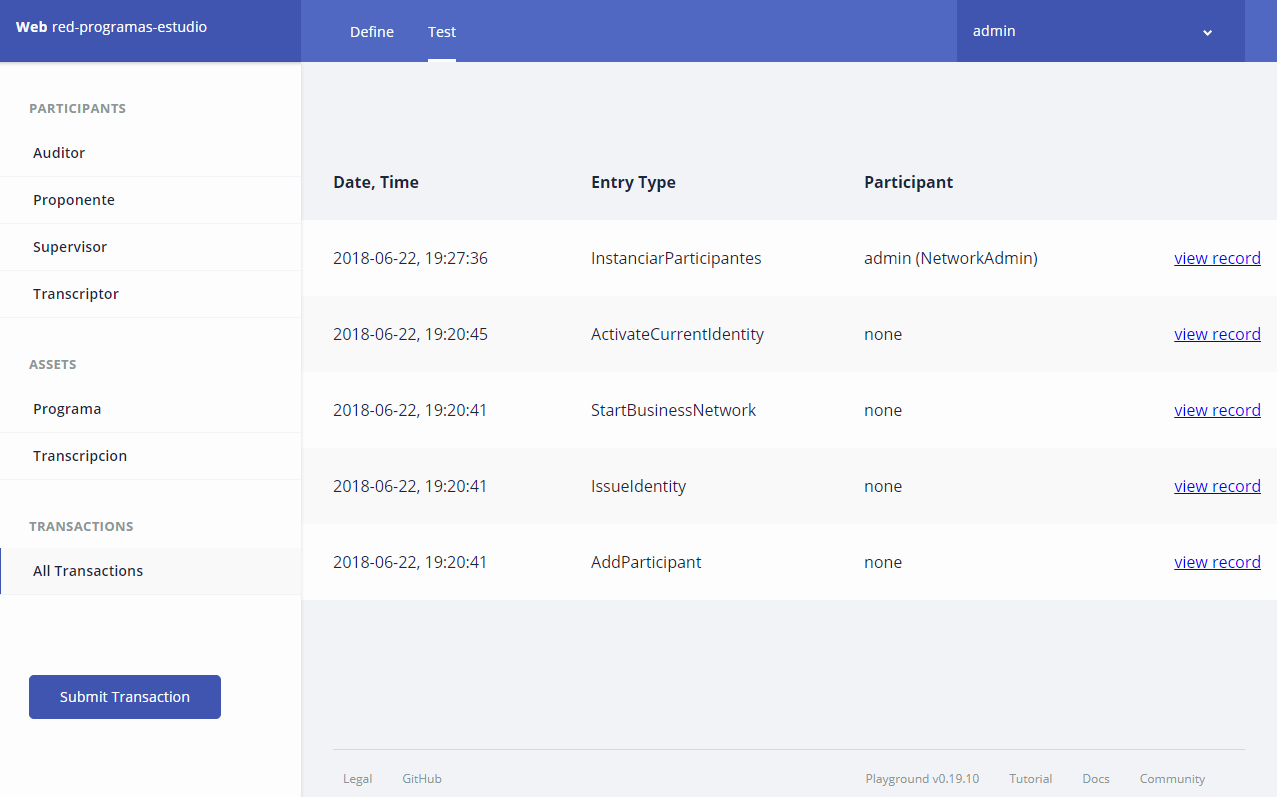
\includegraphics[width=1\textwidth]{playground1.png}
\caption[Interface Playground]{Interfaz gráfica  de Playground.}
\label{fig: playground-presentation}
\end{figure}

La funcionalidad principal del playground se resume en 2 pestañas principales, \textit{Test} y \textit{Define}, ubicadas en la esquina superior izquierda de la interfaz y se muestran en la figura \ref{fig: playground-tabs}. La pestaña \textit{Test} se utiliza para consultar registros, probar transacciones y verificar el  histórico de transacciones realizadas dentro de la red. La pestaña \textit{Define} se utiliza para definir y desarrollar los 3 componentes del modelo de red nombrados a lo largo de todo el capitulo.

\begin{figure}[h]
\centering
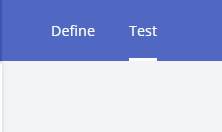
\includegraphics[width=0.5\textwidth]{playground7.png}
\caption[Tabs Playground]{Pestañas de Playground }
\label{fig: playground-tabs}
\end{figure}

El panel izquierdo de la pestaña \textit{Test}  permite visualizar los recursos de la red (\textit{Participantes}, \textit{Activos}, e histórico de \textit{Transacciones}, haciendo click en cualquier de los elementos expuestos en la figura \ref{fig: playground-test-sidebar})
\begin{figure}[H]
\centering
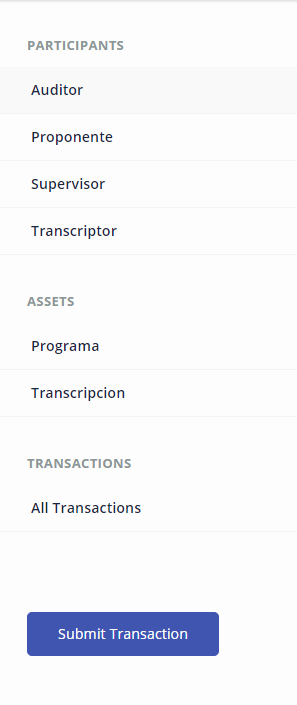
\includegraphics[height=0.5\textheight]{playground2.png}
\caption[Test Sidebar Playground]{Panel lateral de la pestaña \textit{Test} en \textit{Playground} }
\label{fig: playground-test-sidebar}
\end{figure}

En la sección principal de la pestaña \textit{Test},se puede visualizar los diferentes recursos agregados a la red. En la figura \ref{fig: playground-test-principal} se muestran los registros de \textit{Transcripción} \textit{A\_TRANS001} y \textit{A\_TRANS002} cada uno representa la transcripcion de un programa de estudio de la cadena de matemáticas (\textit{Matematicas I }y \textit{Matematicas II} respectivamente).

\begin{figure}[h]
\centering
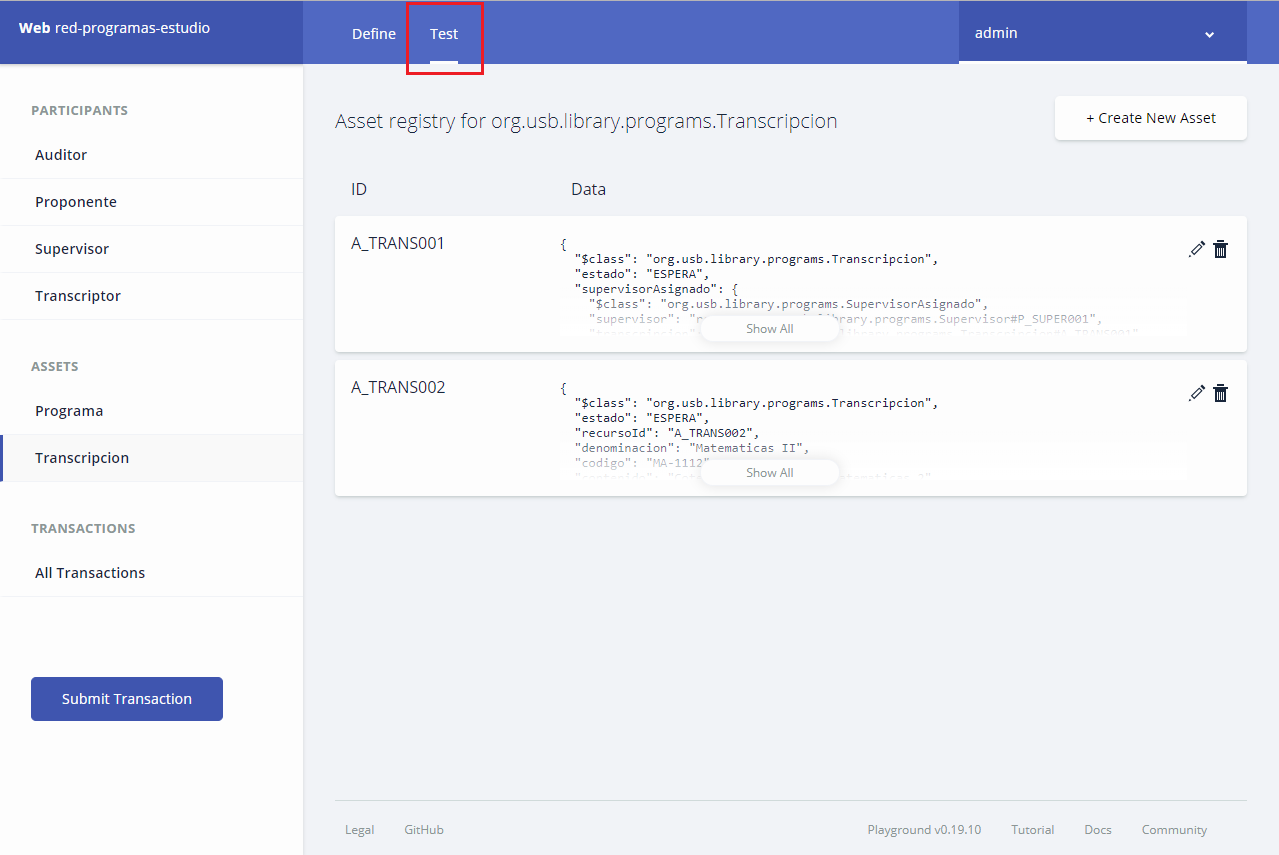
\includegraphics[width=1\textwidth]{playground3.png}
\caption[Test Principal Playground]{Seccion principal de la pestaña \textit{Test} }
\label{fig: playground-test-principal}
\end{figure}

En la figura \ref{fig: playground-test-register} se aprecia un ejemplo de la transcripción en proceso del programa de estudios de \textit{Matemáticas I} (código de materia \textit MA-1111)

\begin{figure}[H]
\centering
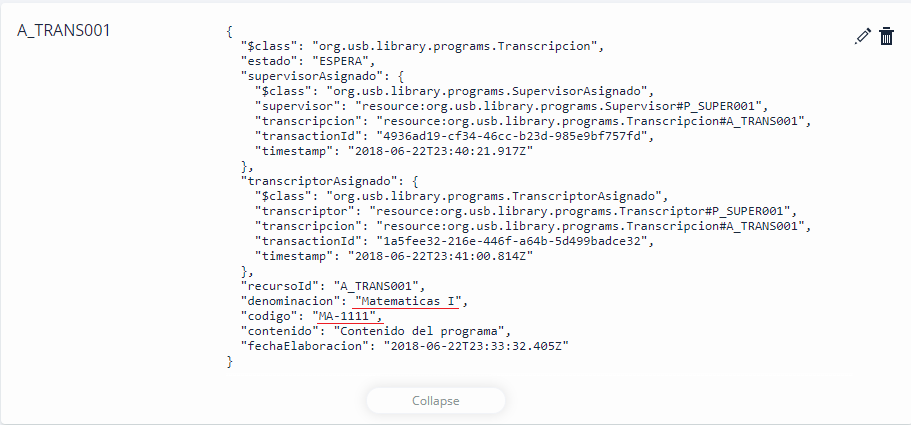
\includegraphics[width=1\textwidth]{playground4.png}
\caption[Test Register Playground]{Vista detalla de un registro de \textit Transcripcion.}
\label{fig: playground-test-register}
\end{figure}

Para la ejecución y prueba de transacciones se utiliza la opción \textit{Submit Transaction} encontrada al final del panel izquierdo de la pestaña \textit{Test} como se muestra en la figura \ref{fig: playground-test-transaction} que también  muestra  las transacciones del modelo descritas en el Capítulo 3.

\begin{figure}[h]
\centering
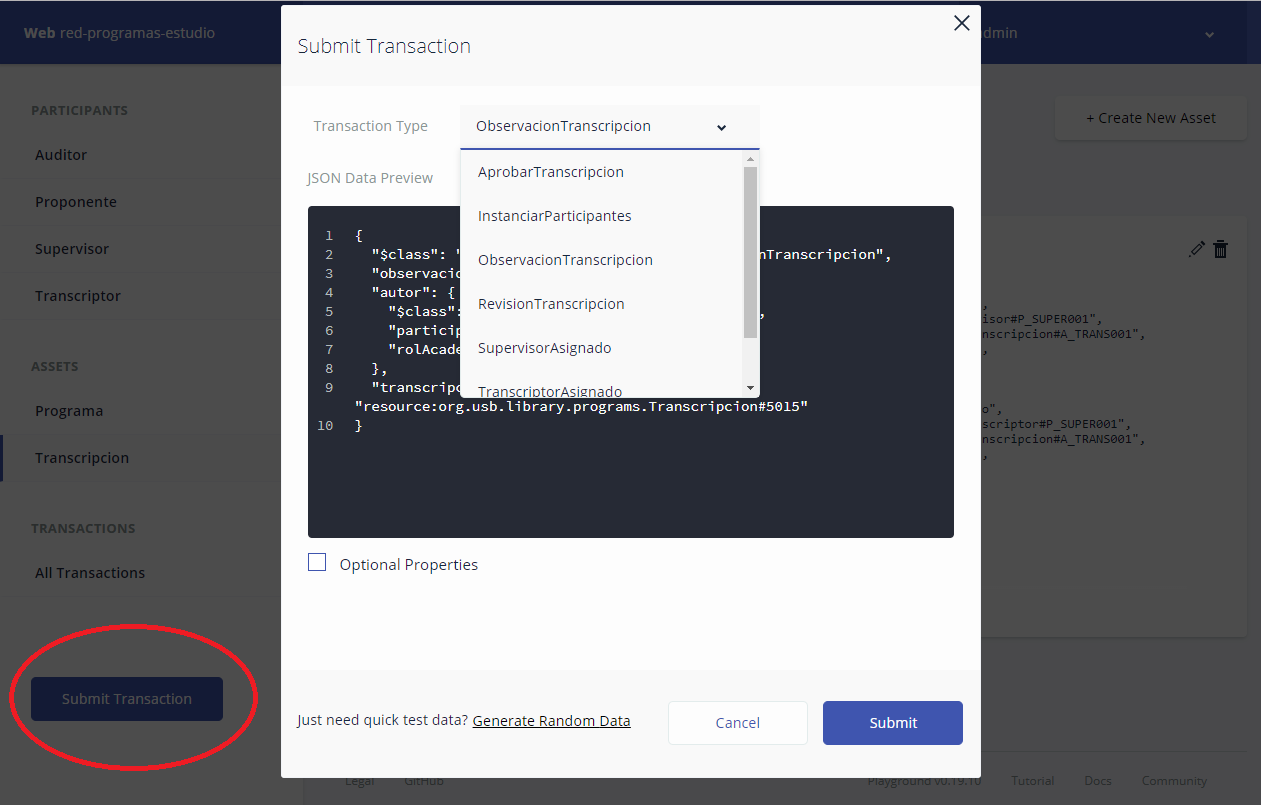
\includegraphics[width=1\textwidth]{playground5.png}
\caption[Test Transaction Playground]{Ventana de prueba y ejecución de transacciones o chaincodes}
\label{fig: playground-test-transaction}
\end{figure}

La pestaña \textit{Define}  permite crear y codificar los archivos necesarios para iniciar el modelo de red. En la figura \ref{fig: playground-define-principal} se expone el editor de texto que provee \textit{Playground} para el desarrollo y visualización de archivos.

\begin{figure}[h]
\centering
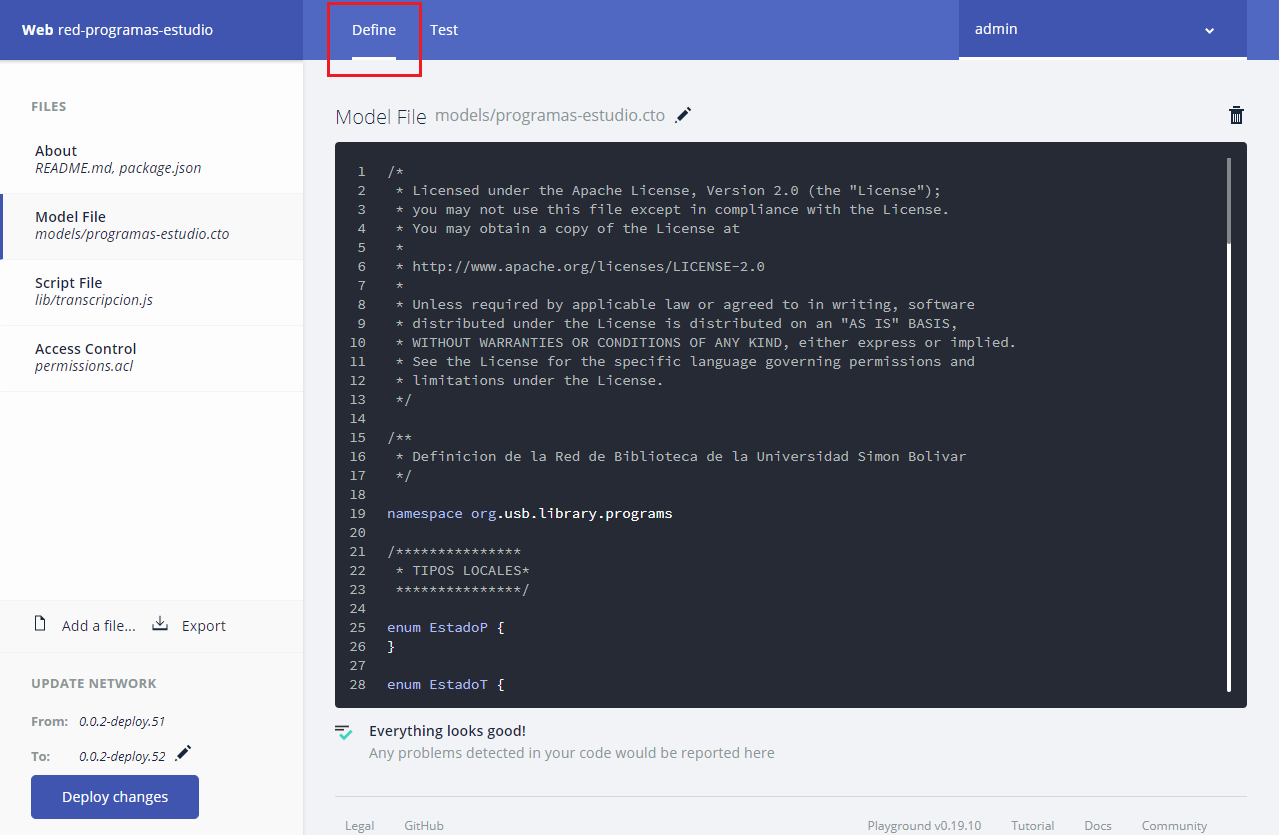
\includegraphics[width=1\textwidth]{playground6.png}
\caption[Define Principal Playground]{Pestaña \textit{Define} vista general.}
\label{fig: playground-define-principal}
\end{figure}

En el panel izquierdo de la pestaña \textit{Define} podemos encontrar los archivos  necesarios del modelo de red. En la figura \ref{fig: playground-define-sidebar} se aprecian los archivos descritos en el capitulo 4: \textit{programas-estudio.cto}, \textit{transcripcion.js}, \textit{permissions.acl}. Todos pueden ser vistos y editados a traves del editor de texto dinamico mencionado anteriormente.
\begin{figure}[H]
\centering
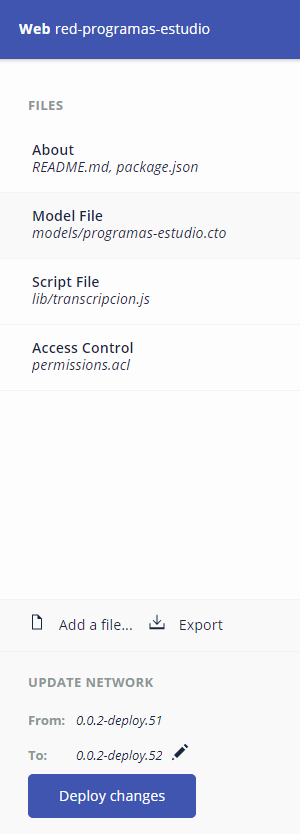
\includegraphics[height=0.6\textheight]{playground8.png}
\caption[Define Sidebar Playground]{Panel lateral de la pestaña \textit{Define}}
\label{fig: playground-define-sidebar}
\end{figure}

Como ilustra la figura \ref{fig: playground-define-export}, las opciones al final del panel permiten agregar archivos locales, desplegar o guardar los cambios y principalmente exportar (crear) el archivo \textit{BNA} necesario para levantar una red blockchain real en \textit{Hyperledger Fabric} como se explica en el capitulo 3.
\begin{figure}[H]
\centering
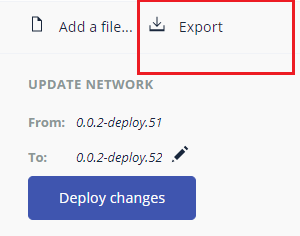
\includegraphics[width=0.3\textwidth]{playground9.png}
\caption[Define Export Playground]{Opcion \textit{Export} al final del panel lateral}
\label{fig: playground-define-export}
\end{figure}

